\uuid{qYoY}
\exo7id{5823}
\titre{exo7 5823}
\auteur{rouget}
\organisation{exo7}
\datecreate{2010-10-16}
\isIndication{false}
\isCorrection{true}
\chapitre{Conique}
\sousChapitre{Hyperbole}
\module{Géométrie}
\niveau{L2}
\difficulte{}

\contenu{
\texte{
Soit $(\mathcal{H})$ une hyperbole équilatère de centre $O$ et $P$ et $Q$ deux points de $(\mathcal{H})$ symétriques par rapport à $O$. Montrer que le cercle de centre $P$ et de rayon $PQ$ recoupe $(\mathcal{H})$ en trois points formant un triangle équilatéral de centre $P$.
}
\reponse{
On peut choisir un repère orthonormé dans lequel $(\mathcal{H})$ admet pour équation équation cartésienne $xy = ab$ et $P$ a pour coordonnées $(a,b)$ où $a$ et $b$ sont deux réels strictement positifs.

$$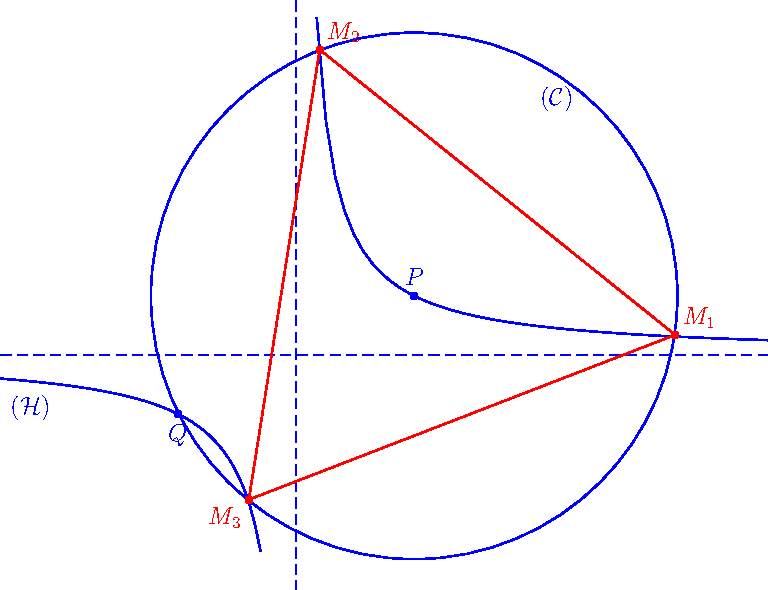
\includegraphics{../images/img005823-1}$$



Le cercle $(\mathcal{C})$ de centre $P$ et de rayon $PQ = 2OP$ admet la paramétrisation $\left\{
\begin{array}{l}
x=a+2\sqrt{a^2+b^2}\cos\theta\\
y=b+2\sqrt{a^2+b^2}\sin\theta
\end{array}
\right.$.

Soit $M(a+2\sqrt{a^2+b^2}\cos\theta,b+2\sqrt{a^2+b^2}\sin\theta)$, $\theta\in\Rr$, un point du cercle $\mathcal{C}$.

\begin{align*}\ensuremath
M(x,y)\in(\mathcal{H})&\Leftrightarrow (a+2\sqrt{a^2+b^2}\cos\theta)(b+2\sqrt{a^2+b^2}\sin\theta) = ab\\
 &\Leftrightarrow(a^2+b^2)\cos\theta\sin\theta + 2\sqrt{a^2+b^2}(b\cos\theta+a\sin\theta) = 0\\
 &\Leftrightarrow\sin(2\theta)+\frac{b}{\sqrt{a^2+b^2}}\cos\theta+\frac{a}{\sqrt{a^2+b^2}}\sin\theta= 0\\
 &\Leftrightarrow\sin(2\theta) +\sin(\theta+\theta_0) = 0\;\text{où}\;\theta_0 =\Arccos\left(\frac{a}{\sqrt{a^2+b^2}}\right)  \\
 &\Leftrightarrow\sin\left(\frac{3\theta+\theta_0}{2}\right)\cos\left(\frac{\theta-\theta_0}{2}\right)=0\Leftrightarrow\theta=\theta_0 +\pi\;(2\pi)\;\text{ou}\;\theta=-\frac{\theta_0}{3}\;\left(\frac{2\pi}{3}\right).
\end{align*}

Les égalités $\theta=\theta_0 +\pi\;(2\pi)$ fournissent le point $Q$.

Les égalités $\theta=-\frac{\theta_0}{3}\;\left(\frac{2\pi}{3}\right)$ fournissent trois valeurs deux à deux distinctes de $\theta$ modulo $2\pi$ et donc trois points deux à deux distincts $M_1$, $M_2$ et $M_3$ de l'hyperbole tels que les trois angles au centre $P$ du triangle $M_1M_2M_3$ soient égaux à $\frac{2\pi}{3}$. Puisque $P$ est le centre du cercle circonscrit à ce triangle, ce triangle est équilatéral de centre $P$.
}
}
